\documentclass{article}
\usepackage{amsmath, amssymb}
\providecommand{\real}[1]{\mathbb{R}}
\usepackage{tikz}
\usetikzlibrary{matrix,positioning,decorations.pathreplacing}
\begin{document}
\section{Gram-Schmidt Orthogonalization}   \label{sec:gram-schmidt}




Given a basis $\{ v_1, \ldots, v_m\}$ of a subspace $S \subset \real^n$, the Gram-Schmidt process
constructs an orthonormal basis $\{ q_1, \ldots, q_m\}$, i.e., basis where the basis vectors satisfy
\[
          q_i^T q_j = \left\{ \begin{array}{ll}
                                       1 & \mbox{ if } i=j, \\
                                       0 & \mbox{ otherwise },
                               \end{array} \right.
\]
of the same subspace $S$.
More precisely, for $k = 1, \ldots, m$ the Gram-Schmidt process successively computes  an orthonormal 
basis $\{ q_1, \ldots, q_k\}$ from $\{ v_1, \ldots, v_k\}$ such that both bases span the same subspace.
The idea is to use orthogonal projection to remove components along the existing basis vectors, 
leaving an orthogonal set. The geometric idea is illustrated in Figure \ref{fig:gram-schmidt-proj}.


\begin{figure}[!h]
\begin{center}
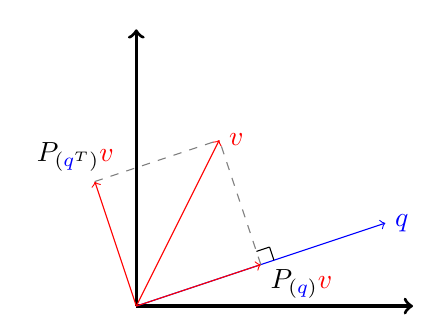
\begin{tikzpicture}
\draw[->,very thick] (0,0) -- +(100pt,0pt);
\draw[->,very thick] (0,0) -- +(0pt,100pt);
\draw[->,blue] (0,0) -- +(90pt,30pt);
\draw[->,red] (0,0) -- +(30pt,60pt);
\draw[->,red] (0,0) -- +(45pt,15pt);
\draw[->,red] (0,0) -- +(-15pt,45pt);
\draw[dashed,gray] (45pt,15pt) -- (30pt,60pt);
\draw[dashed,gray] (-15pt,45pt) -- (30pt,60pt);
\draw (49.7434pt,16.5811pt) -- (48.1623pt,21.3246pt);
\draw (43.4189pt,19.7434pt) -- (48.1623pt,21.3246pt);
\draw (90pt,30pt) node[anchor=west] {${\color{blue} q}$};
\draw (30pt,60pt) node[anchor=west] {${\color{red} v}$};
\draw (45pt,8pt) node[anchor=west] {$P_{\cR({\color{blue} q})}{\color{red} v}$};
\draw (-22pt,45pt) node[anchor=south] {$P_{\cN({\color{blue}
q}^T)}{\color{red} v}$};
\end{tikzpicture}
\end{center}
\caption{The projectors $P_{\cR({\color{blue} q})}={\color{blue}
q}{\color{blue} q}^T/({\color{blue} q}^T{\color{blue} q})$ and
$P_{\cN({\color{blue} q}^T)}=I-P_{\cR({\color{blue} q})}$ decompose
the vector ${\color{red} v}$ into the component $P_{\cR({\color{blue}
q})}{\color{red} v}$ along ${\color{blue} q}$, and the orthogonal
component $P_{\cN({\color{blue} q}^T)}{\color{red} v}$.}
\label{fig:gram-schmidt-proj}
\end{figure}



The steps of the Gram-Schmidt process are described next.
\begin{list}{}{}
\item[$k=1$.]
If $k=1$, then we need to find a vector $q_1$ with $q_1^Tq_1=1$ such that
\[
         \mbox{span} \{ q_1 \} = \mbox{span} \{ v_1 \}.
\]
The vector $q_1$ is obtained by normalizing $v_1$:
\[
        q_1 = v_1 / \|v_1\|_2.
\]

\item[$k=2$.]
Given $q_1$ we want to compute $q_2$ such that $q_1^Tq_2 = 0$, $q_2^Tq_2=1$, and
\[
         \mbox{span} \{ q_1, q_2 \} = \mbox{span} \{ v_1, v_2 \}.
\]
First note that 
since $\mbox{span} \{ q_1 \} = \mbox{span} \{ v_1 \}$ we have $\mbox{span} \{ v_1, v_2 \} = \mbox{span} \{ q_1, v_2 \}$.
Moreover, by the Fundamental Theorem of Linear Algebra we can write $v_2$ as the sum of  vector
in $\mbox{span} \{ q_1 \}  = \cR(Q_1)$, where $Q_1$ is the matrix $Q_1 = (q_1) \in \real^{n\times 1}$, 
and a vector in the orthogonal complement of $\cR(Q_1)$.
We can use projections to express these vectors. The projection onto  $\cR(Q_1)$ is given by
$P_{\cR(Q_1)}= Q_1 (Q_1^TQ_1)^{-1} Q_1^T$. Since $q_1^Tq_1=1$, $Q_1^TQ_1 =1$ and the projection is
given by
\[
         P_{\cR(Q_1)}= Q_1Q_1^T.
\]
Hence,
\[
     v_2 =  Q_1Q_1^T v_2 + (I-Q_1Q_1^T) v_2.
\]
Since $Q_1Q_1^T v_2 \in \cR(Q_1) = \mbox{span} \{ q_1 \}$ we have
\[
       \mbox{span} \{ q_1, v_2 \} =   \mbox{span} \{ q_1, (I-Q_1Q_1^T) v_2 \}.
\]
The vector 
\[
       \widetilde{q}_2 = (I-Q_1Q_1^T) v_2 = v_2 - (q_1^Tv_2) q_1
\]
is orthogonal to $q_1$. We just need to normalize it to obtain 
\[
       q_2 =   \widetilde{q}_2 / \| \widetilde{q}_2 \|_2.
\]
We have
\[
      \mbox{span} \{ v_1, v_2 \} = \mbox{span} \{ q_1, v_2 \} = \mbox{span} \{ q_1, (I-Q_1Q_1^T) v_2 \}
      =   \mbox{span} \{ q_1, q_2 \}
\]

\item[$k>2$.]
Given $q_1, \ldots, q_{k-1}$ with
\[
          q_i^T q_j = \left\{ \begin{array}{ll}
                                       1 & \mbox{ if } i=j, \\
                                       0 & \mbox{ otherwise }.
                               \end{array} \right.
\]
and $\mbox{span} \{ q_1, \ldots, q_{k-1} \} = \mbox{span} \{ v_1,  \ldots, v_{k-1} \}$, we want to compute
$q_k$ such that $q_j^Tq_k = 0$, $j = 1, \ldots, k-1$, $q_k^Tq_k=1$, and
\[
         \mbox{span} \{ q_1, \ldots, q_{k-1}, q_k \} = \mbox{span} \{ v_1,  \ldots, v_{k-1}, v_k \}.
\]
Since $\mbox{span} \{ q_1, \ldots, q_{k-1}  \} = \mbox{span} \{ v_1,  \ldots, v_{k-1} \}$ we have 
\[
         \mbox{span} \{ v_1,  \ldots, v_{k-1}, v_k \} = \mbox{span} \{ q_1, \ldots, q_{k-1}, v_k \}.
\]
By the Fundamental Theorem of Linear Algebra we can write $v_k$ as the sum of  vector
in $\mbox{span} \{  q_1, \ldots, q_{k-1}  \}  = \cR(Q_{k-1})$, where $Q_{k-1}$ is the matrix 
$Q_{k-1} = ( q_1, \ldots, q_{k-1}) \in \real^{n\times k-1}$, 
and a vector in the orthogonal complement of $\cR(Q_{k-1})$.
We can use projections to express these vectors. The projection onto  $\cR(Q_{k-1})$ is given by
$P_{\cR(Q_{k-1})}= Q_{k-1} (Q_{k-1}^TQ_{k-1})^{-1} Q_{k-1}^T$. Since the columns
$q_1, \ldots, q_{k-1}$ of $Q_{k-1}$ are orthonormal, $Q_{k-1}^TQ_{k-1} =I$ and the projection is
given by
\[
         P_{\cR(Q_{k-1})}= Q_{k-1}Q_{k-1}^T.
\]
Hence,
\[
     v_k =  Q_{k-1}Q_{k-1}^T v_k + (I-Q_{k-1}Q_{k-1}^T) v_k.
\]
Since $Q_1Q_1^T v_2 \in \cR(Q_1) = \mbox{span} \{ q_1 \}$ we have
\[
       \mbox{span} \{ q_1, \ldots, q_{k-1}, v_2 \} =   \mbox{span} \{ q_1, \ldots, q_{k-1},  (I-Q_{k-1}Q_{k-1}^T) v_k\}.
\]
The vector 
\[
       \widetilde{q}_k =  (I-Q_{k-1}Q_{k-1}^T) v_k  = v_k - \sum_{j=1}^{k-1} (q_j^Tv_k) q_j
\]
is orthogonal to $ q_1, \ldots, q_{k-1}$. We just need to normalize it to obtain 
\[
       q_k =   \widetilde{q}_k / \| \widetilde{q}_k \|_2.
\]
We have
\begin{align*}
             \mbox{span} \{ v_1,  \ldots, v_{k-1}, v_k \} 
             &= \mbox{span} \{ q_1, \ldots, q_{k-1}, v_k \}
             =  \mbox{span} \{ q_1, \ldots, q_{k-1},  (I-Q_{k-1}Q_{k-1}^T) v_k\} \\
             &=   \mbox{span} \{ q_1, \ldots, q_{k-1},  q_k\}.
\end{align*}
\end{list}



%
%\begin{theorem}[Gram-Schmidt]
%Let $\{v_1,v_2,\cdots,v_m\}$ be a basis for the subspace $S\subset \real^n$. Then it is possible to construct an orthonormal basis $\{q_1, q_2, \cdots ,q_m\}$ for $S$ from the basis vectors $v_1,v_2,\cdots,v_m$.
%\end{theorem}
%\begin{proof}
%If $\textrm{dim}(S)=1$, then upon normalization of $v_1$, $\{v_1\}$ constitutes an orthonormal basis. We will assume that it is possible to construct an orthonormal basis $\{q_1,q_2,\cdots,q_{k-1}\}$ for the subspace of $S$ spanned by $\{v_1,v_2,\cdots,v_{k-1}\}$, and then show how to construct an orthonormal basis for $\{v_1,v_2,\cdots,v_k\}$. The proof then concludes by induction. 
%
%Write
%\begin{align}
%q_k=v_k-\sum_{j=1}^{k-1}c_jq_j, \label{eq:gram-schmidt-decomp}
%\end{align}
%with the scalar coefficients $c_j$ not yet determined. Then, take the inner product of \eref{eq:gram-schmidt-decomp} with $q_l$ for some $l<k$ to obtain
%\[ q_l^Tq_k=q_l^Tv_k-\sum_{j=1}^{k-1}c_jq_l^Tq_j. \]
%Inspection of this equation shows that in order to have $q_l^Tq_k=0$, the coefficients must be chosen so that
%\[ c_l=q_l^Tv_k. \]
%It remains to be shown that with $q_k$ so defined, 
%\[ \textrm{span}(\{q_1,q_2,\cdots,q_k\})=\textrm{span}(\{v_1,v_2,\cdots,v_k\}). \]
%Certainly, it holds that
%\[ q_1,q_2,\cdots,q_{k-1}\in \textrm{span}(\{v_1,v_2,\cdots,v_k\}), \]
%as we have by assumption $\textrm{span}(\{q_1,q_2,\cdots,q_{k-1}\})=\textrm{span}(\{v_1,v_2,\cdots,v_{k-1}\})$, so the inclusion still holds with the extra vector $v_k$. By \eref{eq:gram-schmidt-decomp}, we have that $q_k\in \textrm{span}(\{v_1,v_2,\cdots,v_k\})$, and therefore,
%\[ \textrm{span}(\{q_1,q_2,\cdots,q_k\})\subset \textrm{span}(\{v_1,v_2,\cdots,v_k\}). \]
%A similar argument shows containment in the other direction, completing the proof.
%\end{proof}
%
%Note that the proof is constructive, i.e., it gives an explicit algorithm, known as the Gram-Schmidt process, for computing the vectors $q_1, q_2, \cdots ,q_m$ from the vectors $v_1,v_2,\cdots,v_m$. 


We use the Gram-Schmidt method to compute orthonormal eigenvectors, i.e., to compute orthonormal
bases for the eigenspaces  $  {\cal N}(\lambda_j I - A)$.

 
\begin{example}   \label{ex:diag-symmetric-ex1}
  In Example~\ref{ex:eigenvec-distinct-eigenvalues-ex4} we have shown that the  matrix
   \[
      A = \left( \begin{array}{rrr}
                   1   &  1 &    1\\
                   1   &  1 &    1\\
                   1  &   1 &    1
             \end{array} \right)
  \]
  has eigenvalues  $\lambda_1 =0$,  $\lambda_2 =0$,  $\lambda_3 =3$.
  The corresponding eigenspaces, i.e, the nullspaces $  {\cal N}(0I - A)$
  and ${\cal N}(3I - A)$ are
  \begin{align*}
              {\cal N}(0I - A) &= \mbox{span}\Big\{  \left( \begin{array}{r} -1 \\ 1 \\ 0
                                                                             \end{array} \right) ,
                                                                            \left( \begin{array}{r} -1 \\ 0 \\ 1
                                                                             \end{array} \right) \Big \},                           \\
             {\cal N}(3I - A) &= \mbox{span}\Big\{  \left( \begin{array}{r} 1 \\ 1 \\ 1
                                                                      \end{array} \right) \Big \}.       
   \end{align*}
  Furthermore, we have shown that
  \begin{align*} 
        \left( \begin{array}{rrr}
                  1   &  1 &    1\\
                   1   &  1 &    1\\
                   1  &   1 &    1
          \end{array} \right)
   &=    \underbrace{ \left( \begin{array}{rrr}
                    -1 & -1 & 1 \\
                   1 & 0 & 1 \\
                   0 & 1 & 1
          \end{array} \right) }_{=V}
            \underbrace{ \left( \begin{array}{rrr}
                   0   &  0 &    0\\
                   0   &  0 &    0\\
                   0  &   0 &   3
           \end{array} \right) }_{=\Lambda}
           \underbrace{ \left( \begin{array}{rrr}
                  -1/3   & 2/3 &   -1/3\\
                  -1/3    & -1/3 &  2/3\\
                 1/3 & 1/3 & 1/3
          \end{array} \right)  }_{=V^{-1}}.
    \end{align*}
    The matrix $V$ of eigenvectors is invertible, but not orthonormal. This is due to the fact that
    we have computed bases of the  eigenspaces  ${\cal N}(0I - A)$ and  ${\cal N}(3I - A)$, but
    not orthonormal bases.
    
    We can do this now using Gram-Schmidt.
    To compute an orthonormal basis for ${\cal N}(0I - A)$ we proceed as follows.
    Let $v_1 = (-1, 1, 0)^T$ and $v_2 = (-1, 0, 1)^T$. An orthonormal basis is obtained by computing
    \begin{align*}
         q_1 &=  v_1 / \| v_1 \|_2 = \bpm -1 \\ 1 \\ 0 \epm / \sqrt{2}, \\
         \widetilde{q}_2 &=  v_2 - (v_2^T q_1) \; q_1  
                                       =  \bpm -1 \\ 0 \\ 1 \epm  -   \frac{1}{2} \bpm -1 \\ 1 \\ 0 \epm  =   \bpm -1/2 \\ -1/2 \\ 1 \epm , \\
         q_2 &=  \widetilde{q}_2 / \|  \widetilde{q}_2 \| =  \frac{1}{\sqrt{6}} \bpm -1 \\ -1 \\ 2 \epm .
    \end{align*}
    To compute an orthonormal basis  for ${\cal N}(3I - A)$    we just need to normalize the original
    basis vector. The normalized basis vector is 
    \[
           q_3 =  \frac{1}{\sqrt{3}} \bpm 1 \\ 1 \\ 1 \epm.
     \]
    It is easy to verify that the vectors $q_1, q_2, q_3$ are orthogonal.
    
    The vectors $q_1, q_2$ are eigenvectors corresponding to the eigenvalue 0 and the vector $q_3$
    is an eigenvectors corresponding to the eigenvalue 3.
    Hence
     \[
        \left( \begin{array}{rrr}
                  1   &  1 &    1\\
                   1   &  1 &    1\\
                   1  &   1 &    1
          \end{array} \right)
          \underbrace{ \left( \begin{array}{rrr}
                    -1/ \sqrt{2} & -1// \sqrt{6} & 1/\sqrt{3} \\
                   1/ \sqrt{2} & -1// \sqrt{6} & 1/ \sqrt{3} \\
                   0 & 2/ \sqrt{6} & 1/\sqrt{3}
          \end{array} \right) }_{=Q}
    =    \underbrace{ \left( \begin{array}{rrr}
                    -1/ \sqrt{2} & -1// \sqrt{6} & 1/\sqrt{3} \\
                   1/ \sqrt{2} & -1// \sqrt{6} & 1/ \sqrt{3} \\
                   0 & 2/ \sqrt{6} & 1/\sqrt{3}
          \end{array} \right) }_{=Q}
            \underbrace{ \left( \begin{array}{rrr}
                   0   &  0 &    0\\
                   0   &  0 &    0\\
                   0  &   0 &    3
           \end{array} \right) }_{=\Lambda}.
     \]
     Since the matrix $Q$ is orthogonal, $Q^{-1}=Q^T$ and we have
      \[
        \left( \begin{array}{rrr}
                  1   &  1 &    1\\
                   1   &  1 &    1\\
                   1  &   1 &    1
          \end{array} \right)
    =    \underbrace{ \left( \begin{array}{rrr}
                    -1/ \sqrt{2} & -1/ \sqrt{6} & 1/\sqrt{3} \\
                   1/ \sqrt{2} & -1/ \sqrt{6} & 1/ \sqrt{3} \\
                   0 & 2/ \sqrt{6} & 1/\sqrt{3}
          \end{array} \right) }_{=Q}
            \underbrace{ \left( \begin{array}{rrr}
                   0   &  0 &    0\\
                   0   &  0 &    0\\
                   0  &   0 &    3
           \end{array} \right) }_{=\Lambda}
             \underbrace{ \left( \begin{array}{rrr}
                   -1/ \sqrt{2} & 1/ \sqrt{2} & 0 \\
                   -1/ \sqrt{6} & -1/ \sqrt{6} & 2/ \sqrt{6} \\
                    1/\sqrt{3}  & 1/ \sqrt{3} & 1/\sqrt{3}
          \end{array} \right) }_{=Q^T}.
  \]

  If we use Matlab to compute the eigendecomposition of $A$ we obtain
  \begin{verbatim}
>> A = ones(3,3);
>> [Q,Lambda]=eig(A);
>> Q

Q =

    0.4082    0.7071    0.5774
    0.4082   -0.7071    0.5774
   -0.8165         0    0.5774

>> Lambda

Lambda =

   -0.0000         0         0
         0         0         0
         0         0    3.0000
  \end{verbatim}
    Note that the first column in the matrix {\tt Q} computed by Matlab is $-q_2$ and  
    the second column in the matrix {\tt Q} computed by Matlab is $-q_1$.
    Thus, the first two columns in  the matrix {\tt Q} computed by Matlab are just another
    orthonormal basis for  ${\cal N}(0I - A)$.    
\end{example}
\end{document}